\subsection{两条异面直线所成的角}\label{subsec:1-6}

直线 $a$、$b$ 是异面直线。 经过空间任意一点 $O$,分别引直 $a' \pingxing a$, $b' \pingxing b$。
因为两条相交直线和另外两条相交直线分别平行时,两组直线所成的锐角(或直角)相等,
所以直线 $a'$ 和 $b'$ 所成的锐角(或直角)的大小,只由直线 $a$、$b$ 的相互位置来确定,
与点 $O$ 的选择无关。我们把直线 $a'$ 和 $b'$ 所成的锐角(或直角)
叫做\zhongdian{异面直线 $a$ 和 $b$ 所成的角}(图 \ref{fig:ltjh-1-17})。

\begin{figure}[htbp]
    \centering
    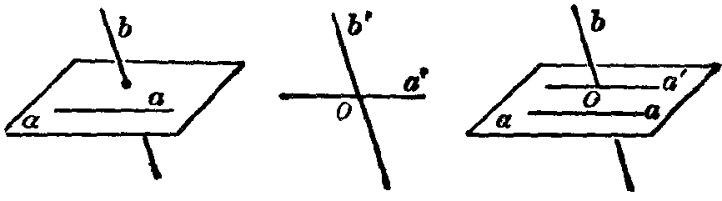
\includegraphics[width=11cm]{../pic/ltjh-ch1-17.png}
    \caption{}\label{fig:ltjh-1-17}
\end{figure}

为了简便,点 $O$ 常取在两条异面直线中的一条上。
例如,取在直线 $b$ 上,然后经过点 $O$ 作直线 $a' \pingxing a$(图 \ref{fig:ltjh-1-17}),
那么 $a'$ 和 $b$ 所成的角就是异面直线 $a$、$b$ 所成的角。

如果两条异面直线所成的角是直角,我们就说这\zhongdian{两条异面直线互相垂直}。

例如,图 \ref{fig:ltjh-1-11} 中,六角螺帽的两条棱 $AB$、$CD$ 所在直线是成 $60^\circ$ 角的异面直线;
蜗轮和蜗杆的轴线是互相垂直的异面直线,它表明由蜗杆到蜗轮的传动方向变了 $90^\circ$ 的角。

\begin{wrapfigure}[8]{r}{5cm}
    \centering
    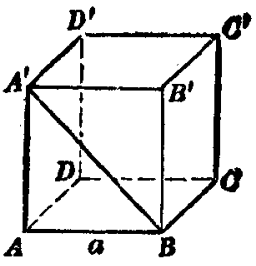
\includegraphics[width=4cm]{../pic/ltjh-ch1-18.png}
    \caption{}\label{fig:ltjh-1-18}
\end{wrapfigure}

图 \ref{fig:ltjh-1-18} 中,正方体的棱 $AA'$ 和 $B'C'$ 所在的直线是两条异面直线,直线 $A'B'$ 和它们都垂直相交。
我们把和两条异面直线都垂直相交的直线叫做\zhongdian{两条异面直线的公垂线}。

两条异面直线的公垂线在这两条异面直线间的线段的长度,叫做\zhongdian{两条异面直线的距离}。
图 \ref{fig:ltjh-1-18} 中线段 $A'B'$ 的长度就是异面直线 $AA'$ 和 $B'C'$ 的距离。

\liti[0] 设图 \ref{fig:ltjh-1-18} 中的正方体的棱长为 $a$。

(1)图中哪些棱所在的直线与直线 $BA'$ 成异面直线?

(2)求直线 $BA'$ 和 $CC'$ 所成的角的大小;

(3)求异面直线 $BC$ 和 $AA'$ 的距离。

\jie (1) $\because$ \quad $A' \not \in \text{平面}\;BC'$,
而点 $B$、直线 $CC'$ 都在平面 $BC'$ 内,且 $B \not \in CC'$。

$\therefore$ \quad 直线 $BA'$ 与 $CC'$ 是异面直线。

同理,直线 $C'D'$、$D'D$、$DC$、$AD$、$B'C'$ 都和直线 $BA'$ 成异面直线。

(2) $\because$ \quad $CC' \pingxing BB'$,

$\therefore$ \quad $BA'$ 和 $BB'$ 所成的锐角就是 $BA'$ 和 $CC'$ 所成的角。

$\because$ \quad $\angle A'BB' = 45^\circ$,

$\therefore$ \quad $BA'$ 和 $CC'$ 所成的角是 $45^\circ$。

(3) $\because$ \quad $AB \perp AA'$, $AB \cap AA' = A$,

又\quad $\because$ \quad $AB \perp BC$, $AB \cap BC = B$,

$\therefore$ \quad $AB$ 是 $BC$ 和 $AA'$ 的公垂线段。

$\because$ \quad $AB = a$,

$\therefore$ \quad $BC$ 和 $AA'$ 的距离是 $a$。


\begin{lianxi}

\xiaoti{}%
\begin{xiaoxiaotis}%
    \xxt[\xxtsep]{两条直线互相垂直,它们一定相交吗?}

    \xxt{垂直于同一直线的两条直线,有几种位置关系?}

\end{xiaoxiaotis}

\xiaoti{举出互相垂直的异面直线和异面直线的公垂线的实际例子。}

\xiaoti{画两个相交平面,在这两个平面内各画一条直线使它们成为
    (1)平行直线; (2)相交直线; (3)异面直线。
}

\end{lianxi}

